\documentclass[12pt, a4paper, twoside]{article}
\usepackage[utf8]{inputenc}
\usepackage{fancyhdr}
\usepackage{graphicx}
\usepackage{caption}
\usepackage{subcaption}
\usepackage[margin=1in,footskip=0.25in]{geometry}
\usepackage{pgf}
\usepackage[absolute, overlay]{textpos}
\usepackage{pdfpages}
\usepackage[siunitx]{circuitikz}
\usepackage{adjustbox}
\usepackage{pgfplots}

\pgfplotsset{width=10cm, compat=1.9}

\setlength{\TPHorizModule}{1.0 pt}
\textblockorigin{\paperwidth}{0.0 pt}

\pagestyle{fancy}
\fancyhf{}
\lhead{Stromkreise \& Glühlampchen}
\rhead{Physik Kurzbericht}
\begin{document}
    \pgfmathwidth{"\\\\ J. Dubois \& A. Huillet\\ MNG Rämibühl\\"}
    \begin{textblock}{\pgfmathresult}[1, 0](0, 0)
    \noindent
    \\\\ J. Dubois \& A. Huillet\\ MNG Rämibühl\\ 8001 Zürich
    \end{textblock}
    \begin{titlepage}

    \begin{center}
        \vspace*{8cm}
        \Huge
        \textbf{Stromkreise \& Glühlampchen}
 
        \vspace{0.5cm}
        \LARGE
        Physik Bericht  
    \end{center}
    \vspace*{8cm}
    \normalsize
    \hspace*{2cm}Physik Bericht mit Bezug auf das Praktikum vom 24. März 2022\\\\
    \hspace*{2cm}Zürich, 7. April 2022
    
             
 \end{titlepage}

    \newpage
    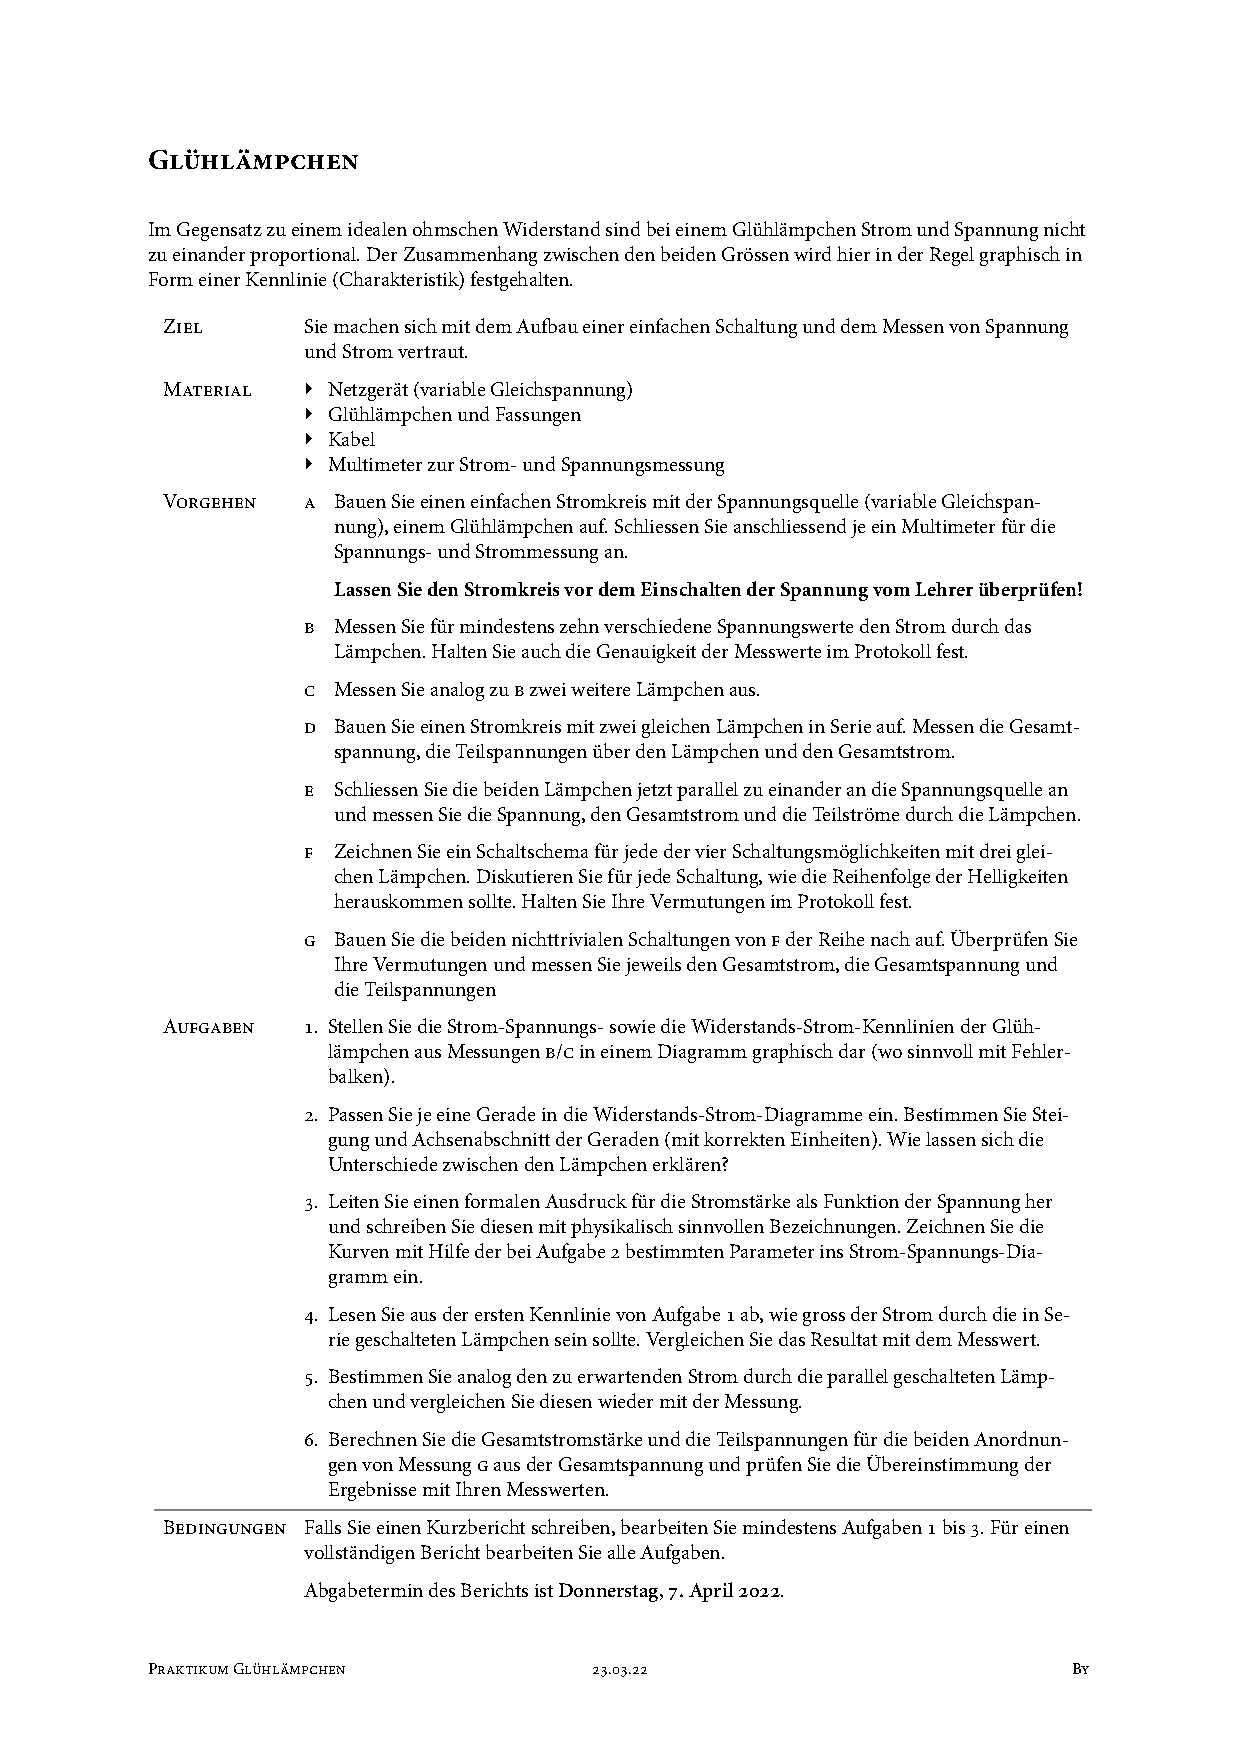
\includepdf[pages=-]{aufgabenstellung.pdf}
    \section{Experiment}
    \newpage
    \section{Messungen}     
    \subsection{Messung A}
    Ein einfacher Stromkreis wurde gebaut. Dieser wird für die Messungen A, B und C\\ benutzt:\\
    \newline
    \begin{center}
        \begin{adjustbox}{scale=0.4}
            \begin{circuitikz} \draw
                (0,10) to[vsource, i=\LARGE{$I$}, l_=\LARGE{$U$}] (0,0)
                (0,10) to[lamp, l=\LARGE{$U_1$},i=\LARGE{$I_1$}] (16,10)--(16,0)--(0,0)
                ;
            \end{circuitikz}        
        \end{adjustbox}
        \end{center}
    \subsection{Messung B}
    Bei Messung B wurden für zehn verschiedenen Spannungswerte den Strom durch das Lämpchen gemessen:\\
    \begin{center}
        \begin{tabular}{l|r}
            \textbf{Spannung U[V]} & \textbf{Stromstärke I[mA]}\\
            \hline
            3.65 & 39.50\\
            5.11 & 48.30\\
            8.33 & 64.60\\
            10.37 & 73.60\\
            12.50 & 82.20\\
            15.54 & 93.60\\
            17.62 & 100.70\\
            19.74 & 107.70\\
            23.80 & 120.00\\
            24.85 & 123.00
        \end{tabular}
    \end{center}
    \subsection{Messung C}
    In dieser Messung wurde das gleiche Verfahren wie bei Messung B bei zwei weiteren Lämpchen angewendet.
    \newpage
    \textbf{Messung für Lämpchen 2:}\\
    \begin{center}
        \begin{tabular}{l|r}
            \textbf{Spannung U[V]} & \textbf{Stromstärke I[mA]}\\
            \hline
            3.65 & 39.10\\
            5.11 & 48.40\\
            8.33 & 64.00\\
            10.37 & 73.30\\
            12.50 & 81.80\\
            15.54 & 93.60\\
            17.62 & 101.00\\
            19.74 & 107.90\\
            23.80 & 120.70\\
            24.85 & 123.90
        \end{tabular}
    \end{center}
    \vspace{1cm}
    \textbf{Messung für Lämpchen 3:}\\
    \begin{center}
        \begin{tabular}{l|r}
            \textbf{Spannung U[V]} & \textbf{Stromstärke I[mA]}\\
            \hline
            3.65 & 39.30\\
            5.11 & 48.50\\
            8.33 & 64.10\\
            10.37 & 73.30\\
            12.50 & 81.70\\
            15.54 & 93.40\\
            17.62 & 100.10\\
            19.74 & 107.10\\
            23.80 & 119.60\\
            24.85 & 122.80
        \end{tabular}
    \end{center}
    \subsection{Messung D}
    Folgender Stromkreis wurde aufgebaut:
    \begin{center}
        \begin{adjustbox}{scale=0.4}
            \begin{circuitikz} \draw
                (0,10) to[vsource, i=\LARGE{$I_{tot}$}, l_=\LARGE{$U_{tot}$},invert] (0,0)
                (0,10) -- (4, 10)
                (4,10) to[lamp, l=\LARGE{$U_1$}, i=\LARGE{$I_1$}] (8,10)
                (8,10) to[lamp, l=\LARGE{$U_2$}, i=\LARGE{$I_2$}] (12,10)
                (12,10)--(16,10) -- (16,0) -- (0,0)
                ;
            \end{circuitikz}  
        \end{adjustbox}
    \end{center}
    \newpage
    Folgende Werte ergaben sich:
    \begin{itemize}
        \item[\LARGE{-}] $U_{tot} = 20.81 V$
        \item[\LARGE{-}] $U_1 = 10.37 mA$
        \item[\LARGE{-}] $U_2 = 10.45 V$
        \item[\LARGE{-}] $I_1 = 73.57 mA$
        \item[\LARGE{-}] $I_2 = 73.6 mA$
        \item[\LARGE{-}] $I_{tot} = 73.6 mA$
        
    \end{itemize}
    \subsection{Messung E}
    Folgender Stromkreis wurde aufgebaut:
    \begin{center}
        \begin{adjustbox}{scale=0.4}
        \begin{circuitikz} \draw
            (0,10) to[vsource,l_=\LARGE{$U_{tot}$}, i=\LARGE{$I_{tot}$}, invert] (0,0)
            (0,10)--(16/3,10)
            (16/3,10)--(16/3,12)
            (16/3,10)--(16/3,8)
            (16/3,12) to[lamp, i=\LARGE{$I_1$}, l=\LARGE{$U_1$}] (32/3,12)
            (16/3,8) to[lamp, i=\LARGE{$I_2$}, l=\LARGE{$U_2$}] (32/3,8)
            (32/3,12)--(32/3,10)
            (32/3,8)--(32/3,12)
            (32/3,10)--(16,10)
            (16,10)--(16,0)--(0,0)
            ;
        \end{circuitikz}
    \end{adjustbox}
    \end{center}
    Die Gesamtspanung $U_{tot}$ und der Gesamtstrom $I_tot$ sind bekannt:
        \[U_{tot} = 20.59 V\]
        \[I_{tot} = 220.6 mA\]
    \newline
    Man weiss schon, dass:
    \[U_1 = U_2 = U_{tot}\]
    \newline
    Das Multimeter zur Strommessung mass folgende Werte für $I_1$ und $I_2$:
        \[I_1 = 111.3 mA \]
        \[I_2 = 110.5 mA\]
    \subsection{Messung F}
    1)
    \begin{center}
        \begin{adjustbox}{scale=0.4}
            \begin{circuitikz}\draw
                (0,10) to[vsource, l_=\LARGE{$U_{tot}$}, i_=\LARGE{$I_{tot}$}] (0,0)
                (0,10) to[lamp, l=\LARGE{$U_1$}, i=\LARGE{$I_1$}] (16/3,10) 
                (16/3,10) to[lamp, l=\LARGE{$U_2$}, i=\LARGE{$I_2$}] (32/3,10)
                (32/3,10) to[lamp, l=\LARGE{$U_3$}, i=\LARGE{$I_3$}] (16,10)
                (16,10)--(16,0)--(0,0)
                ;
            \end{circuitikz}
        \end{adjustbox}
    \end{center}
    2)
    \begin{center}
        \begin{adjustbox}{scale=0.4}
            \begin{circuitikz}\draw
                (0,10) to[vsource, invert, l_=\LARGE{$U_{tot}$}, i_=\LARGE{$I_{tot}$}] (0,0)
                (0,10)--(4,10)
                (4,10)--(4,11)
                (4,10)--(4,9)
                (4,11) to[lamp, l=\LARGE{$U_1$}, i=\LARGE{$I_1$}] (8,11)
                (4,9) to[lamp, l_=\LARGE{$U_2$}, i_=\LARGE{$I_2$}] (8,9)
                (8,11)--(8,10)
                (8,9)--(8,10)
                (8,10) to[lamp, l=\LARGE{$U_3$}, i=\LARGE{$I_3$}] (16,10)
                (16,10)--(16,0)--(0,0)
                ;
            \end{circuitikz}
        \end{adjustbox}
    \end{center}
    3)
    \begin{center}
        \begin{adjustbox}{scale=0.4}
            \begin{circuitikz}\draw
                (0,10) to[vsource, invert, l_=\LARGE{$U_{tot}$}, i_=\LARGE{$I_{tot}$}] (0,0)
                (0,10) to[lamp, l_=\LARGE{$U_1$}, i_=\LARGE{$I_1$}] (8,10)
                (8,10) to[lamp, l_=\LARGE{$U_3$}, i_=\LARGE{$I_3$}] (16,10)
                (4,10.4)--(4,11)
                (4,11) to[lamp, l=\LARGE{$U_2$}, i=\LARGE{$I_2$}] (12,11)
                (12,11)--(12,10.4)
                (16,10)--(16,0)--(0,0)
                ;
            \end{circuitikz}            
        \end{adjustbox}
    \end{center}
    4)
    \begin{center}
        \begin{adjustbox}{scale=0.4}
            \begin{circuitikz}\draw
                (0,10) to[vsource, invert, l_=\LARGE{$U_{tot}$}, i_=\LARGE{$I_{tot}$}] (0,0)
                (0,10)--(4,10)
                (4,10) to[lamp, l=\LARGE{$U_2$}, i=\LARGE{$I_2$}] (12,10)
                (4,10)--(4,12)
                (4,10)--(4,8)
                (12,10)--(12,12)
                (12,10)--(12,8)
                (4,12) to[lamp, l=\LARGE{$U_3$}, i=\LARGE{$I_3$}] (12,12)
                (4,8) to[lamp, l=\LARGE{$U_1$}, i=\LARGE{$I_1$}] (12,8)
                (12,10)--(16,10)
                (16,10)--(16,0)--(0,0)
                ;
            \end{circuitikz}
        \end{adjustbox}
    \end{center}
    Unsere Vermutungen (Helligkeit):
    \begin{enumerate}
        \item 1, 1, 1
        \item 0, 0, 1
        \item $\frac{1}{2}$, 1, $\frac{1}{2}$
        \item 1, 1, 1
    \end{enumerate}
    \subsection{Messung G}
    Folgende Helligkeiten ergaben sich nach dem Bau der Schaltungen von \textbf{Messung F}:
    \begin{enumerate}
        \item $\frac{1}{3}$, $\frac{1}{3}$, $\frac{1}{3}$
        \item 0, 0, 1
        \item $\frac{1}{2}$, 1, $\frac{1}{2}$
        \item 1, 1, 1
    \end{enumerate}
    Folgende Messwerte wurden gemessen:
    \begin{center}
        \begin{tabular}{l|l|l|c|r|r}
            \textbf{Schaltschema} & \textbf{$U_1$} & \textbf{$U_2$} & \textbf{$U_3$} & \textbf{$I_{tot}$} & \textbf{$U_{tot}$}\\
            \hline
            \textbf{1} & 4.196 \textit{V} & 4.100 \textit{V} & 4.250 \textit{V} & 42.500 \textit{mA} & 12.530 \textit{V} \\
            \textbf{2} & 0 \textit{V} & 0 \textit{V} & 12.480 \textit{V} & 81.200 \textit{mA} & 12.480 \textit{V} \\
            \textbf{3} & 6,235 \textit{V} & 12.400 \textit{V} & 6.169 \textit{V} & 155.2 \textit{mA} & 12.400 \textit{V} \\
            \textbf{4} & 12.430 \textit{V} & 12.430 \textit{V} & 12.430 \textit{V} & --Kein Wert-   - & 12.430 \textit{V}

        \end{tabular}
    \end{center}
    \newpage
    \section{Aufgaben}
    \subsection{Aufgabe 1}
    Kennlinien der Glühlämpchen:
    \vspace{1cm}\\
    \begin{tikzpicture}
        \begin{axis}[
            title={\textbf{Strom-Spannungs-Kennlinie}},
            xmin=0, xmax=140,
            ymin=0, ymax=30,
            xlabel = {$I [mA]$},
            ylabel = {$U [V]$},
            legend pos=outer north east,
            axis lines = left,
        ]
        \addplot[
            color=green,
            mark=square*,
        ]
        coordinates{
            (39.3,3.65)(48.4,5.11)(64.23,8.33)(73.4,10.37)(81.9,12.5)
            (93.53,15.54)(100.6,17.62)(107.57,19.74)(120.1,23.8)(123.23,24.85)
        };
        \addlegendentry{$I$-$U$-Kennlinie}
        \end{axis}
    \end{tikzpicture}
    \vspace{2cm}\\
    \begin{tikzpicture}
        \begin{axis}[
            title={\textbf{Widerstands-Strom-Kennlinie}},
            xmin=0, xmax=140,
            ymin=0, ymax=250,
            xlabel = {$I [mA]$},
            ylabel = {$R [\Omega]$},
            legend pos=outer north east,
            axis lines = left,
        ]
        \addplot[
            color=blue,
            mark=square*,
        ]
        coordinates{
            (39.3, 92.88)(48.4, 105.58)(64.233, 129.69)(73.4, 141.281)
            (81.9, 152.626)(93.533, 166.144)(100.6, 175.152)(107.5667, 183.516)
            (120.1, 198.171)(123.233, 201.653)
        };
        \addlegendentry{$R$-$I$-Kennlinie}                 
        \end{axis}
    \end{tikzpicture}
    \vspace{1cm}\\
    Für die Strom-Spannungs-Kennlinie wurden das Mittelwert der Spannung für jede Messung von jedem Glühlämpchen,
    sowie das Mittelwert der Stromstärken für jede Messung von jedem Glühlämpchen berechnet.\\
    \newline
    Für die Widerstands-Strom-Kennlinie wurden das Mittelwert der Stromstärken für jede Messung von jedem Glühlämpchen
    und das Mittelwert der Widerständen für jede Messung von jedem Glühlämpchen berechnet.
    
    \subsection{Aufgabe 2}
    Für die Geraden der Glühlämpchen wurden die Messwerten als Koordinatenpunkte in einer Grafik eingefügt. Somit ergaben sich folgende Grafiken:
    \vspace{1cm}\\
    \begin{tikzpicture}
        \begin{axis}[
            title={Gerade des \textbf{Glühlämpchens 1}},
            xmin=0, xmax=140,
            ymin=0, ymax=250,
            xlabel = {$I [mA]$},
            ylabel = {$R [\Omega]$},
            legend pos=outer north east,
            axis lines = left,
        ]
        \addplot[
            color=purple,
            mark=square*,
            ]
            table{GL1.txt};
        \addlegendentry{Glühlämpchen 1}    
        \end{axis}
    \end{tikzpicture}
    \vspace{1cm}\\
    \begin{tikzpicture}
        \begin{axis}[
            title={Gerade des \textbf{Glühlämpchens 1} im Vergleich zur \textbf{R-I-Kennlinie}},
            xmin=0, xmax=140,
            ymin=0, ymax=250,
            xlabel = {$I [mA]$},
            ylabel = {$R [\Omega]$},
            legend pos=outer north east,
            axis lines = left,
        ]
        \addplot[
            color=purple,
            mark=square*,
            ]
            table{GL1.txt};
        \addlegendentry{Glühlämpchen 1}
        \addplot[
            color=blue,
            mark=square*,
        ]
        coordinates{
            (39.3, 92.88)(48.4, 105.58)(64.233, 129.69)(73.4, 141.281)
            (81.9, 152.626)(93.533, 166.144)(100.6, 175.152)(107.5667, 183.516)
            (120.1, 198.171)(123.233, 201.653)
        };
        \addlegendentry{$R$-$I$-Kennlinie}
            
        \end{axis}
    \end{tikzpicture}
    \vspace{1cm}\\
    \begin{tikzpicture}
        \begin{axis}[
            title={Gerade des \textbf{Glühlämpchens 2}},
            xmin=0, xmax=140,
            ymin=0, ymax=250,
            xlabel = {$I [mA]$},
            ylabel = {$R [\Omega]$},
            legend pos=outer north east,
            axis lines = left,
        ]
            
            \addplot[
                color=red,
                mark=square*,
            ]
            coordinates{(39.1, 93.33)(48.4, 105.5785)(64,130.1563)(73.3, 141.4734)
            (81.8, 152.8117)(93.6, 166.0256)(101, 174.4554)(107.9, 182.9472)
            (120.7, 197.1831)(123.9, 200.565)};
            \addlegendentry{Glühlämpchen 2}
        \end{axis}
    \end{tikzpicture}
    \vspace{1cm}\\
    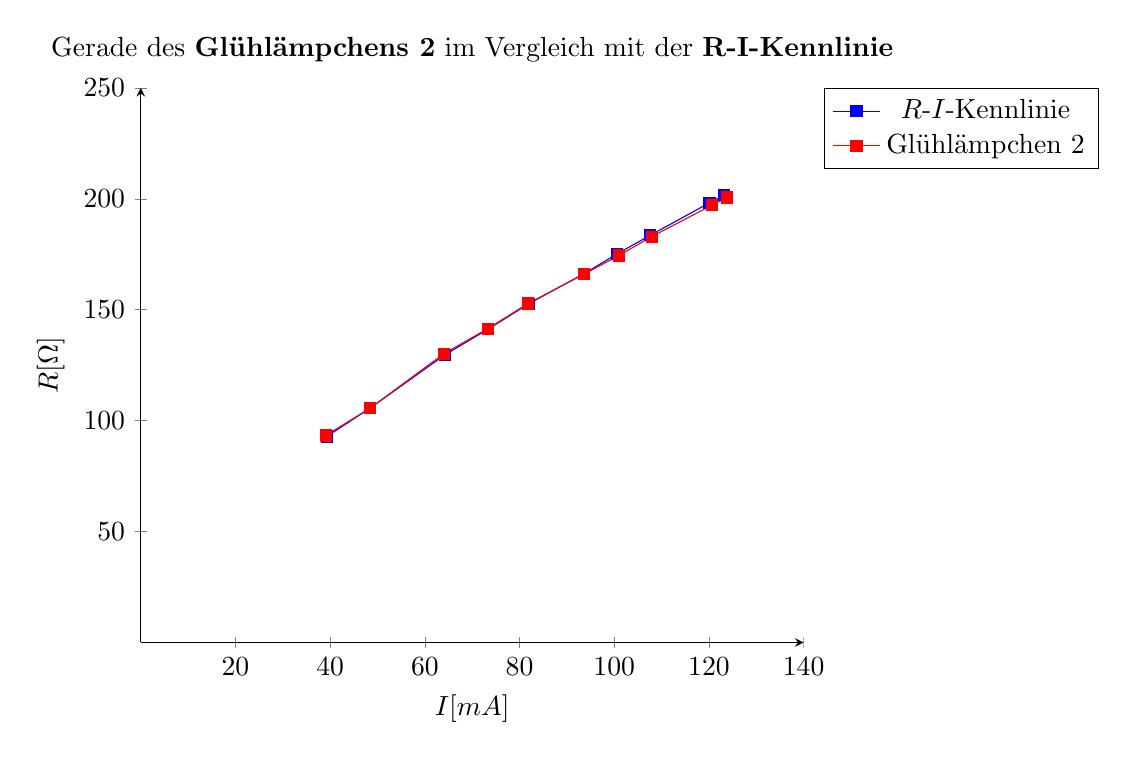
\begin{tikzpicture}
        \begin{axis}[
            title={Gerade des \textbf{Glühlämpchens 2} im Vergleich mit der \textbf{R-I-Kennlinie}},
            xmin=0, xmax=140, 
            ymin=0, ymax=250,
            xtick={20,40,60,80,100,120,140},
            ytick={50,100,150,200, 250},
            xlabel = {$I [mA]$},
            ylabel = {$R [\Omega]$},
            legend pos=outer north east,
            axis lines = left,
        ]

        \addplot[
            color=blue,
            mark=square*,
        ]
        coordinates{
            (39.3, 92.88)(48.4, 105.58)(64.233, 129.69)(73.4, 141.281)
            (81.9, 152.626)(93.533, 166.144)(100.6, 175.152)(107.5667, 183.516)
            (120.1, 198.171)(123.233, 201.653)
        };
        \addlegendentry{$R$-$I$-Kennlinie}      

        \addplot [
            color=red,
            mark=square*,
        ] coordinates{(39.1, 93.33)(48.4, 105.5785)(64,130.1563)(73.3, 141.4734)
        (81.8, 152.8117)(93.6, 166.0256)(101, 174.4554)(107.9, 182.9472)
        (120.7, 197.1831)(123.9, 200.565)};
        \addlegendentry{Glühlämpchen 2}
        \end{axis}        
    \end{tikzpicture}
    \vspace{1cm}\\
    \begin{tikzpicture}
        \begin{axis}[
            title={Gerade des \textbf{Glühlämpchens 3}},
            xmin=0, xmax=140,
            ymin=0, ymax=250,
            xlabel = {$I [mA]$},
            ylabel = {$R [\Omega]$},
            legend pos=outer north east,
            axis lines = left,
        ]
            
            \addplot [
                color=magenta,
                mark=square*,
            ]
            table {GL3.txt};
            \addlegendentry{Glühlämpchen 3}
        \end{axis}
    \end{tikzpicture}
    \vspace{1cm}\\
    \begin{tikzpicture}
        \begin{axis}[
            title={Gerade des \textbf{Glühlämpchens 3} im Vergleich mit der \textbf{R-I-Kennlinie}},
            xmin=0, xmax=140,
            ymin=0, ymax=250,
            xlabel = {$I [mA]$},
            ylabel = {$R [\Omega]$},
            legend pos=outer north east,
            axis lines = left,
        ]
        \addplot [
                color=magenta,
                mark=square*,
            ]
            table {GL3.txt};
            \addlegendentry{Glühlämpchen 3}
            
        \addplot[
            color=blue,
            mark=square*,
        ]
        coordinates{
            (39.3, 92.88)(48.4, 105.58)(64.233, 129.69)(73.4, 141.281)
            (81.9, 152.626)(93.533, 166.144)(100.6, 175.152)(107.5667, 183.516)
            (120.1, 198.171)(123.233, 201.653)
        };
        \addlegendentry{$R$-$I$-Kennlinie}
        \end{axis}
    \end{tikzpicture}
    \newpage
    \subsection{Aufgabe 3}
    Die Spannung bezeichnet die Arbeit pro Ladung:
    \begin{equation}
        U = \frac{W}{Q}
    \end{equation}
    Die Stromstärke bezeichnet die Anzahl Ladungen pro Zeit:
    \begin{equation}
        I = \frac{Q}{t}
    \end{equation}
    Die Leistung bezeichnet die Arbeit pro Zeit:
    \begin{equation}
        P = \frac{W}{t}
    \end{equation}
\end{document}
